% Desenvolvido por: Prof. Dr. David Buzatto
%
% Versão 1.6.3
% Data: 04/12/2023

\documentclass[
	12pt,
   	oneside,
   	a4paper,
   	chapter=TITLE,
   	english,
   	french,
   	spanish,
   	brazil,
]{abntex2}

\usepackage{estrutura}

% ---
% Dados do documento
% ---

\tipotrabalho{Relatório Técnico}

\titulo{Desenvolvimento de um cozy game 2D na engine Godot.}
% caso não haja, comente a linha abaixo
%\subtitulo{subtítulo (se houver)}

\autor{Bianca Emily Lourenço}
\orientador{Prof.Dr.David Buzzato}
% caso não haja, comente a linha abaixo
%\coorientador{Prof./Profa. Me./Dr./Dra. Nome Completo}

\curso{Bacharelado em Ciência da Computação}
\grau{Bacharel em Ciência da Computação}

%exemplos
%\curso{Bacharelado em Ciência da Computação}
%\grau{Bacharel em Ciência da Computação em Sistemas para Internet}
%\curso{Especialização em Desenvolvimento de Aplicações para Dispositivos Móveis}
%\grau{Especialista em Desenvolvimento de Aplicações para Dispositivos Móveis}

\campus{São João da Boa Vista}
\area{Engenharia de Software}

\local{São João da Boa Vista}
\mes{Abril}
\ano{2025}

\instituicao{%
	Instituto Federal de Educação, Ciência e Tecnologia de São Paulo
	\par
	Câmpus \imprimircampus
}

\preambulo{\imprimirtipotrabalho\ elaborado conforme a ABNT NBR 10719:10, apresentado ao Instituto Federal de Educação, Ciência e Tecnologia de São Paulo, como parte dos requisitos para a obtenção do grau de \imprimirgrau.
\\
\\
Área de Concentração: \imprimirarea}

\setlength{\parindent}{1.3cm}
\setlength{\parskip}{0.2cm}

\makeindex

% ---------------------------------------------------------------------------------
%                                   INÍCIO DO DOCUMENTO
% ---------------------------------------------------------------------------------
\begin{document}
	

% Seleciona o idioma do documento
\selectlanguage{brazil}

% Retira espaço extra obsoleto entre as frases.
\frenchspacing 

\pretextual
\begin{center}
   	
   	\ABNTEXchapterfont\Large\textsc{\imprimirautor}
   	\vspace{2.5cm}
   	
   	\ABNTEXchapterfont\LARGE\textsc{\imprimirtitulo\ifdef{\osubtitulo}{:}{}}

    \ifdef{\osubtitulo}{\ABNTEXchapterfont\Large\imprimirsubtitulo}{}
   	\vspace{2.5cm}
   	   	
   	\hspace{.4\textwidth}
   	\begin{minipage}{.5\textwidth}
   		\SingleSpacing
   		\large\imprimirpreambulo
   		
   		\vspace{\onelineskip}
   		
   		Orientador: \imprimirorientador
   		
        \ifdef{\ocoorientador}{
            \vspace{\onelineskip}
               		
       		Coorientador: \imprimircoorientador
        }{}
        
        
   		
   	\end{minipage}%
    \vfill
   	
   	\Large\textsc{\imprimirlocal}
   	
   	\Large\textsc{\imprimirano}
   	
   	\vspace*{2cm}
   	
\end{center}
\newcommand{\specialcell}[2][c]{%
	\begin{tabular}[#1]{@{}c@{}}#2\end{tabular}}

\FloatBarrier
\begin{table}[!htbp]
	\centering
	\renewcommand{\arraystretch}{1.5}% Spread rows out...
	\begin{tabular}{| >{\centering}m{2in} | >{\centering}m{2in} | >{\centering\arraybackslash}m{2in} | }
		\hline
		\specialcell[t]{INSTITUTO FEDERAL DE\\EDUCAÇÃO, CIÊNCIA E\\TECNOLOGIA DE SÃO\\PAULO - CÂMPUS SÃO\\JOÃO DA BOA VISTA} & \imprimirmes & \imprimirano \\
		\hline
		\multicolumn{3}{|c|}{\specialcell{
				
				\\ \\
				
				\imprimircurso
				
				\\ \\ \\ \\ \\ \\
				
				\begin{minipage}[t]{0.9\columnwidth}%
				    \centering
				    \ABNTEXchapterfont\LARGE\imprimirtitulo\ifdef{\osubtitulo}{:}{}
                    
                    \ifdef{\osubtitulo}{\ABNTEXchapterfont\Large\imprimirsubtitulo}{}
                    
				\end{minipage}
				
				\\ \\ \\ \\
				
				}}\\
		\multicolumn{3}{|r|}{\specialcell{
				
                \begin{minipage}[t]{0.9\columnwidth}%
   				    \flushright
    				\imprimirautor \ifdef{\ocoorientador}{,}{\ e}
                    \\
                    \imprimirorientador \ifdef{\ocoorientador}{ e\\\imprimircoorientador}{}
                \end{minipage}
				
				\\ \\ \\ \\ \\ \\ \\ \\ \\ \\ 
				
			}}\\
			\hline%                                        todas em letras minúsculas, separadas por ponto e vírgula (;)
		\multicolumn{2}{|l|}{\specialcell{Palavras-chave:\\\textit{Cozy Game}. \textit{Godot}. 2D. Jogos.}} & \the\numexpr \getpagerefnumber{LastPage} - 1 \relax \  páginas \\
		\hline
	\end{tabular}
\end{table}
\FloatBarrier

% ---
% Inserir a ficha catalográfica
% ---
%
% Este é um exemplo de ficha catalográfica.
%
% A ficha catalográfica final deve ser requisitada pelo aluno e inserida neste
% documento para a entrega da versão final.
%

\begin{fichacatalografica}
    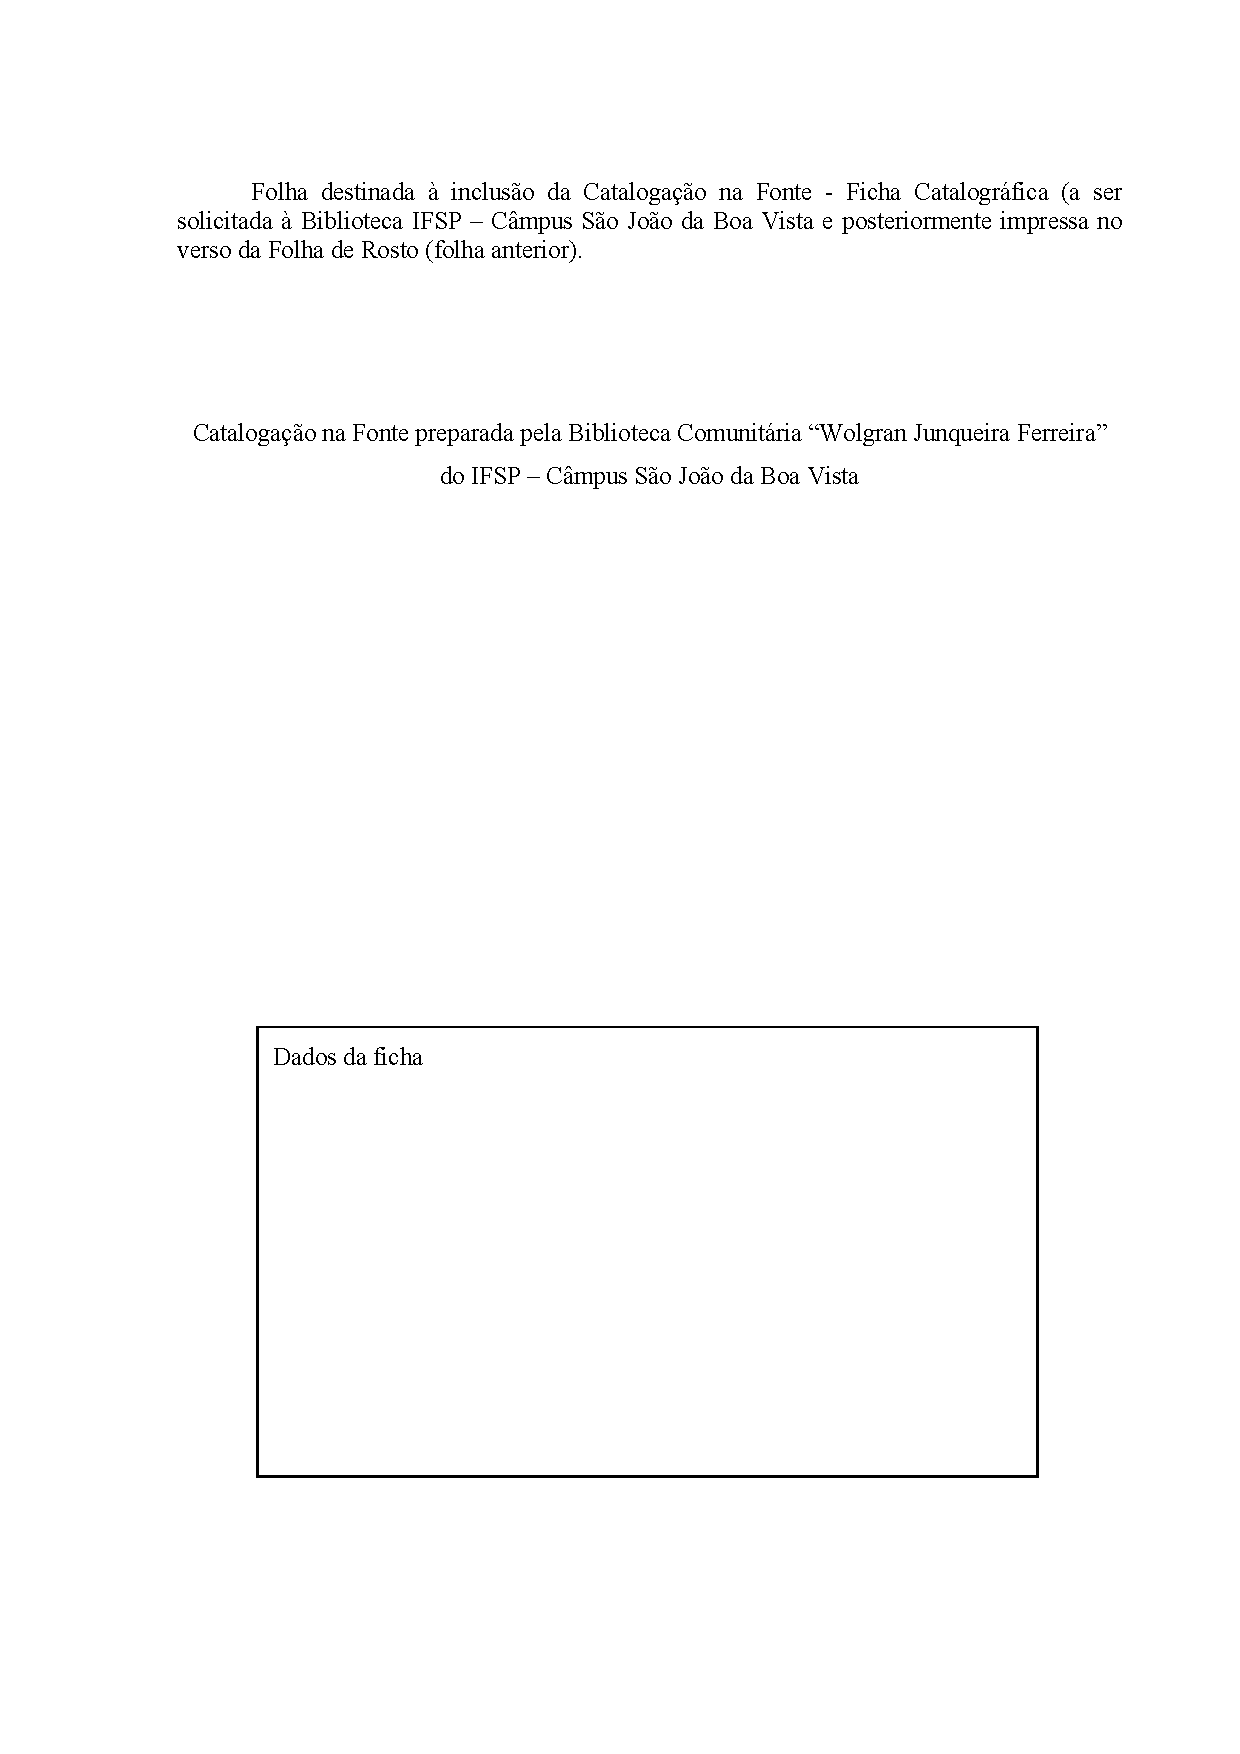
\includepdf{fichaCatalografica/exemploFichaCatalografica.pdf}
\end{fichacatalografica}

% ---
% Inserir ata de defesa
% ---
%
% Este é um exemplo da ata de defesa.
%
% A ata de defesa será fornecida pelo professor orientador após a defesa do trabalho
% e o orientado será responsável em substituir o arquivo de exemplo pelo arquivo final.
%
\begin{folhadeaprovacao}
	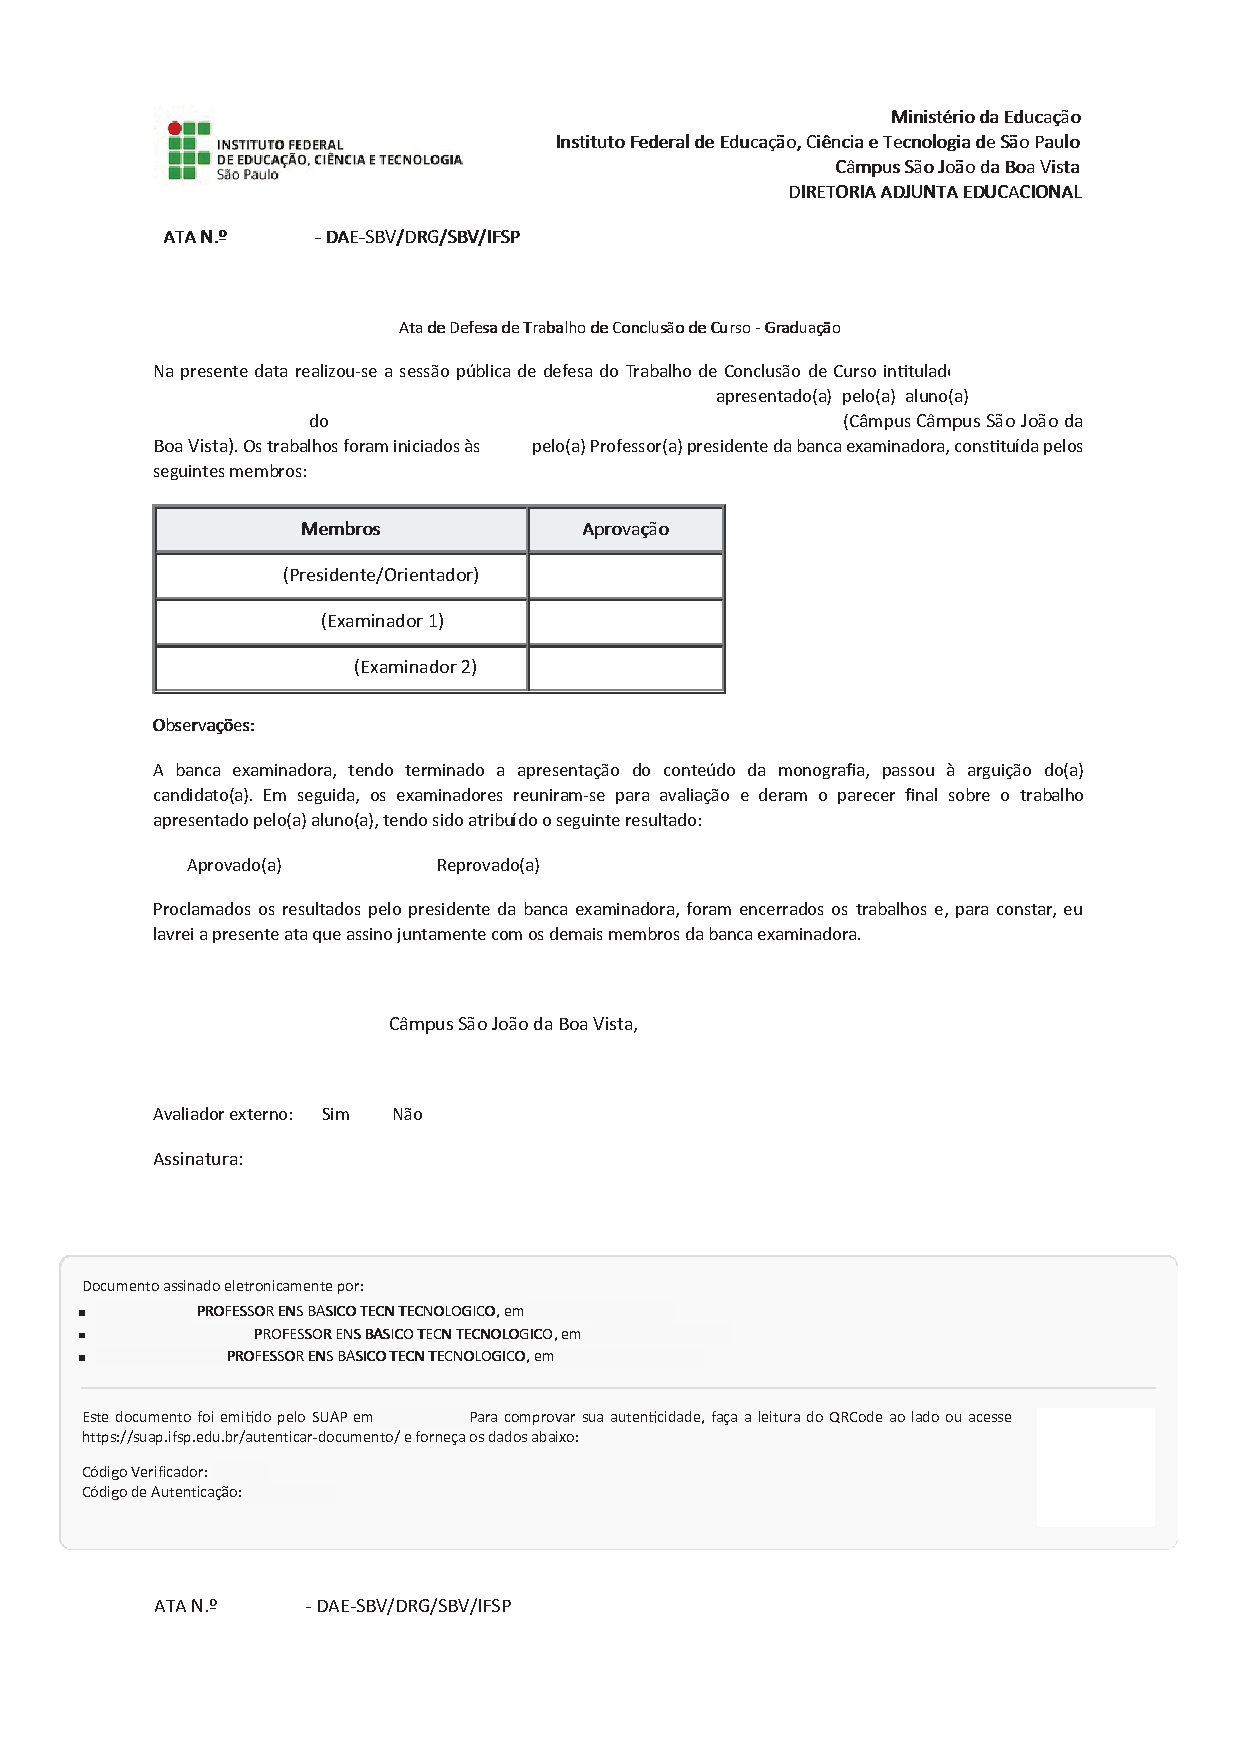
\includepdf[pages={1-}]{ataDefesa/exemploAtaDefesa.pdf}
\end{folhadeaprovacao}

% ---
% inserir o sumário
% ---
\pdfbookmark[0]{\contentsname}{toc}
\tableofcontents*
\cleardoublepage
% ---

\chapter*{}
\noindent{\textbf{RESUMO}}

\noindent{Neste trabalho é apresentada a formatação que deve ser utilizada nos relatórios técnicos a serem submetidos ao final dos cursos de Graduação e Pós-graduação do IFSP câmpus São João da Boa Vista. Leia com atenção este documento. O máximo de palavras para o resumo é 150 (cento e cinquenta).}

\vspace{\onelineskip}

% todas em letras minúsculas, separadas por ponto e vírgula (;)
\noindent{\textbf{Palavras-chave}: palavra-chave 1. palavra-chave 2. palavra-chave 3. palavra-chave n.}

\textual
\chapter{Introdução}
\label{cap:01}

O objetivo deste documento é esclarecer aos autores o formato que deve ser utilizado nos relatórios técnicos a serem submetidos ao final dos cursos de Graduação e Pós-Graduação do IFSP câmpus São João da Boa Vista. Este documento está escrito de acordo com o modelo indicado para a formatação dos relatórios técnicos; assim, serve de referência, ao mesmo tempo em que comenta os diversos aspectos da formatação.

Observe as instruções e formate seu relatório técnico de acordo com este padrão. Lembre-se que uma formatação correta contribui para uma boa avaliação do seu trabalho.

Além disso, neste documento estão listadas as seções obrigatórias que você deverá fornecer, bem como os exemplos dos comandos mais comuns que serão utilizados na construção de seu documento. Para pesquisar sobre mais comandos, recomenda-se a utilização do site \url{https://ctan.org/}, que é a biblioteca principal do \LaTeX, e o do site \url{https://tex.stackexchange.com} que é uma das principais comunidades para solução de dúvidas relacionadas a \LaTeX. Ambas são em inglês.

A introdução é um elemento preliminar, opcional, utilizado para fornecer informações específicas, comentar tecnicamente o conteúdo do trabalho, além de evidenciar as motivações que levaram o autor à escolha de determinado tema.

Trata-se de importante estratégia de aproximação, pois permite valorizar a escolha do assunto, mostrar a relevância da abordagem temática e esclarecer quanto ao passo-a-passo utilizado na estruturação do texto.

Na introdução, o leitor terá condições de avaliar:

\begin{itemize}
	\item O grau de informação, conhecimento e competência técnica do autor relativamente ao assunto a ser tratado;
	\item A qualidade, a eficiência, a originalidade e o ineditismo de sua abordagem;
	\item A pertinência das informações apresentadas e a possibilidade de acrescentar algo de novo ao universo conceitual do leitor.
\end{itemize}


\section{Objetivos}

\subsection{Objetivo Geral}

Desenvolver um \textit{cozy game} 2D utilizando a \textit{engine Godot}, com foco em oferecer uma experiência relaxante e imersiva por meio de mecânicas simples, estética acolhedora e narrativa envolvente.

\subsection{Objetivos Específicos}
\begin{itemize}
	\item Definir o estilo visual e narrativo do jogo;
	\item Projetar jogabilidade e interações relaxantes;
	\item Preparar o ambiente de desenvolvimento na \textit{Godot};
	\item Criar ou adquirir os \textit{assets} visuais e sonoros;
	\item Programar as mecânicas e sistemas do jogo.
	
\end{itemize}
\chapter{Considerações Gerais}
\label{cap:02}

\section{O que é um jogo?}

Segundo o designer de jogos \citeauthorandyear{Crawford1997}, para compreender os jogos e seu design, deve-se primeiramente definir o que se quer representar com a palavra "jogo", a qual ele define como sendo um sistema fechado que representa subjetivamente um subconjunto da realidade. Essa afirmação descreve um jogo como algo completo e autossuficiente, com regras bem definidas que determinam seu funcionamento.

Além disso, o autor identifica quatro elementos fundamentais presentes em todos os jogos. O primeiro é a representação, pois considera que todo jogo sempre reflete, de alguma maneira, aspectos da realidade, mesmo que de forma abstrata ou fantasiosa. O segundo é a interação, pois os jogadores influenciam o jogo ao tomarem decisões. O terceiro é o conflito, que se manifesta por meio de desafios e competição. Por fim, há a segurança, já que as consequências do jogo raramente impactam a realidade.


Já \citeauthorandyear{Suits1978}, filósofo canadense conhecido por seu trabalho sobre a natureza dos jogos, apresenta uma definição mais voltada para o ato de jogar, na qual determina que jogar um jogo é se envolver voluntariamente a uma atividade para alcançar um estado específico, aceitando seguir regras limitantes. Ele também introduz o conceito de \textit{lusory attitude}, que consiste nos jogadores se submeterem a desafios desnecessários para tornar o jogo possível. 



\citeauthorandyear{Crawford1997} define os tipos distintos de jogos, caracterizados a seguir.



\subsection{Jogos de Tabuleiro}

Primeiramente, temos os jogos de tabuleiro, que consistem em uma superfície dividida em setores, os quais são ocupados por um conjunto de peças que, nas configurações comuns, estão diretamente associadas aos jogadores, que as movimentam pelo tabuleiro com o objetivo de capturar as peças do adversário. Um exemplo popular desse tipo de jogo é o Xadrez, que se destaca como um dos jogos de estratégia mais clássicos e influentes, representando bem a essência dos jogos de tabuleiro.

Na Figura~\ref{fig:xadrez}, é ilustrado um tabuleiro de Xadrez com suas peças no começo de uma partida.


\FloatBarrier
\begin{figure}[!htbp]
	\centering
	\caption{Tabuleiro de Xadrez e suas peças}
	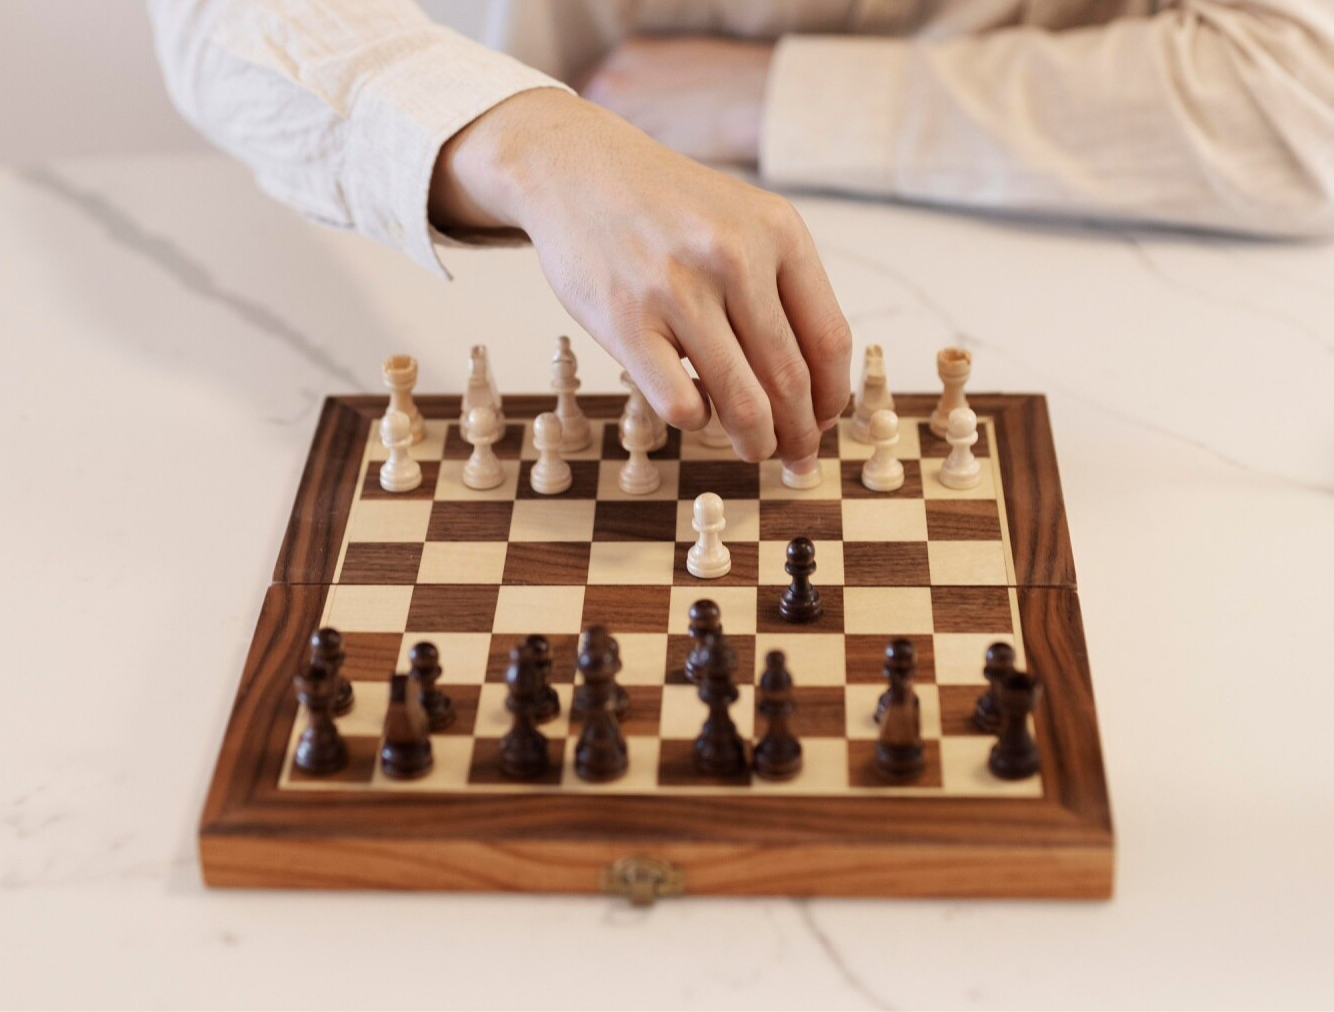
\includegraphics[width=0.7\linewidth]{imagens/Xadrez.png}
	\\\textbf{Fonte:} Freepik
	\label{fig:xadrez}
\end{figure}
\FloatBarrier

\subsection{Jogos de Cartas}

Uma segunda classe de jogos são os jogos de carta, que utilizam um baralho composto por 52 cartas, divididos entre quatro naipes e treze fileiras. O uso do baralho varia conforme o objetivo do jogo, e uma das razões pelas quais os jogos de cartas são tão fascinantes é seu equilíbrio entre sorte e habilidade, diferente dos jogos totalmente aleatórios, como os dados, ou puramente estratégicos, como o xadrez \cite{Parlett1990}.


Segundo \citeauthorandyear{Parlett1990} as cartas possuem uma característica dupla que influencia diretamente a dinâmica dos jogos: a aleatoriedade, que ocorre porque são embaralhadas antes do jogo, e o sigilo, já que apenas o jogador que as possui pode ver seu valor. A questão de sorte nos jogos de cartas está frequentemente ligada à probabilidade, permitindo assim utilizar cálculos matemáticos para prever e influenciar resultados ao longo das partidas. 

Na Figura~\ref{fig:cartas} são apresentadas as cartas presentes em um baralho.


\FloatBarrier 
\begin{figure}[!htbp]
	\centering
	\caption{Cartas de um baralho}
	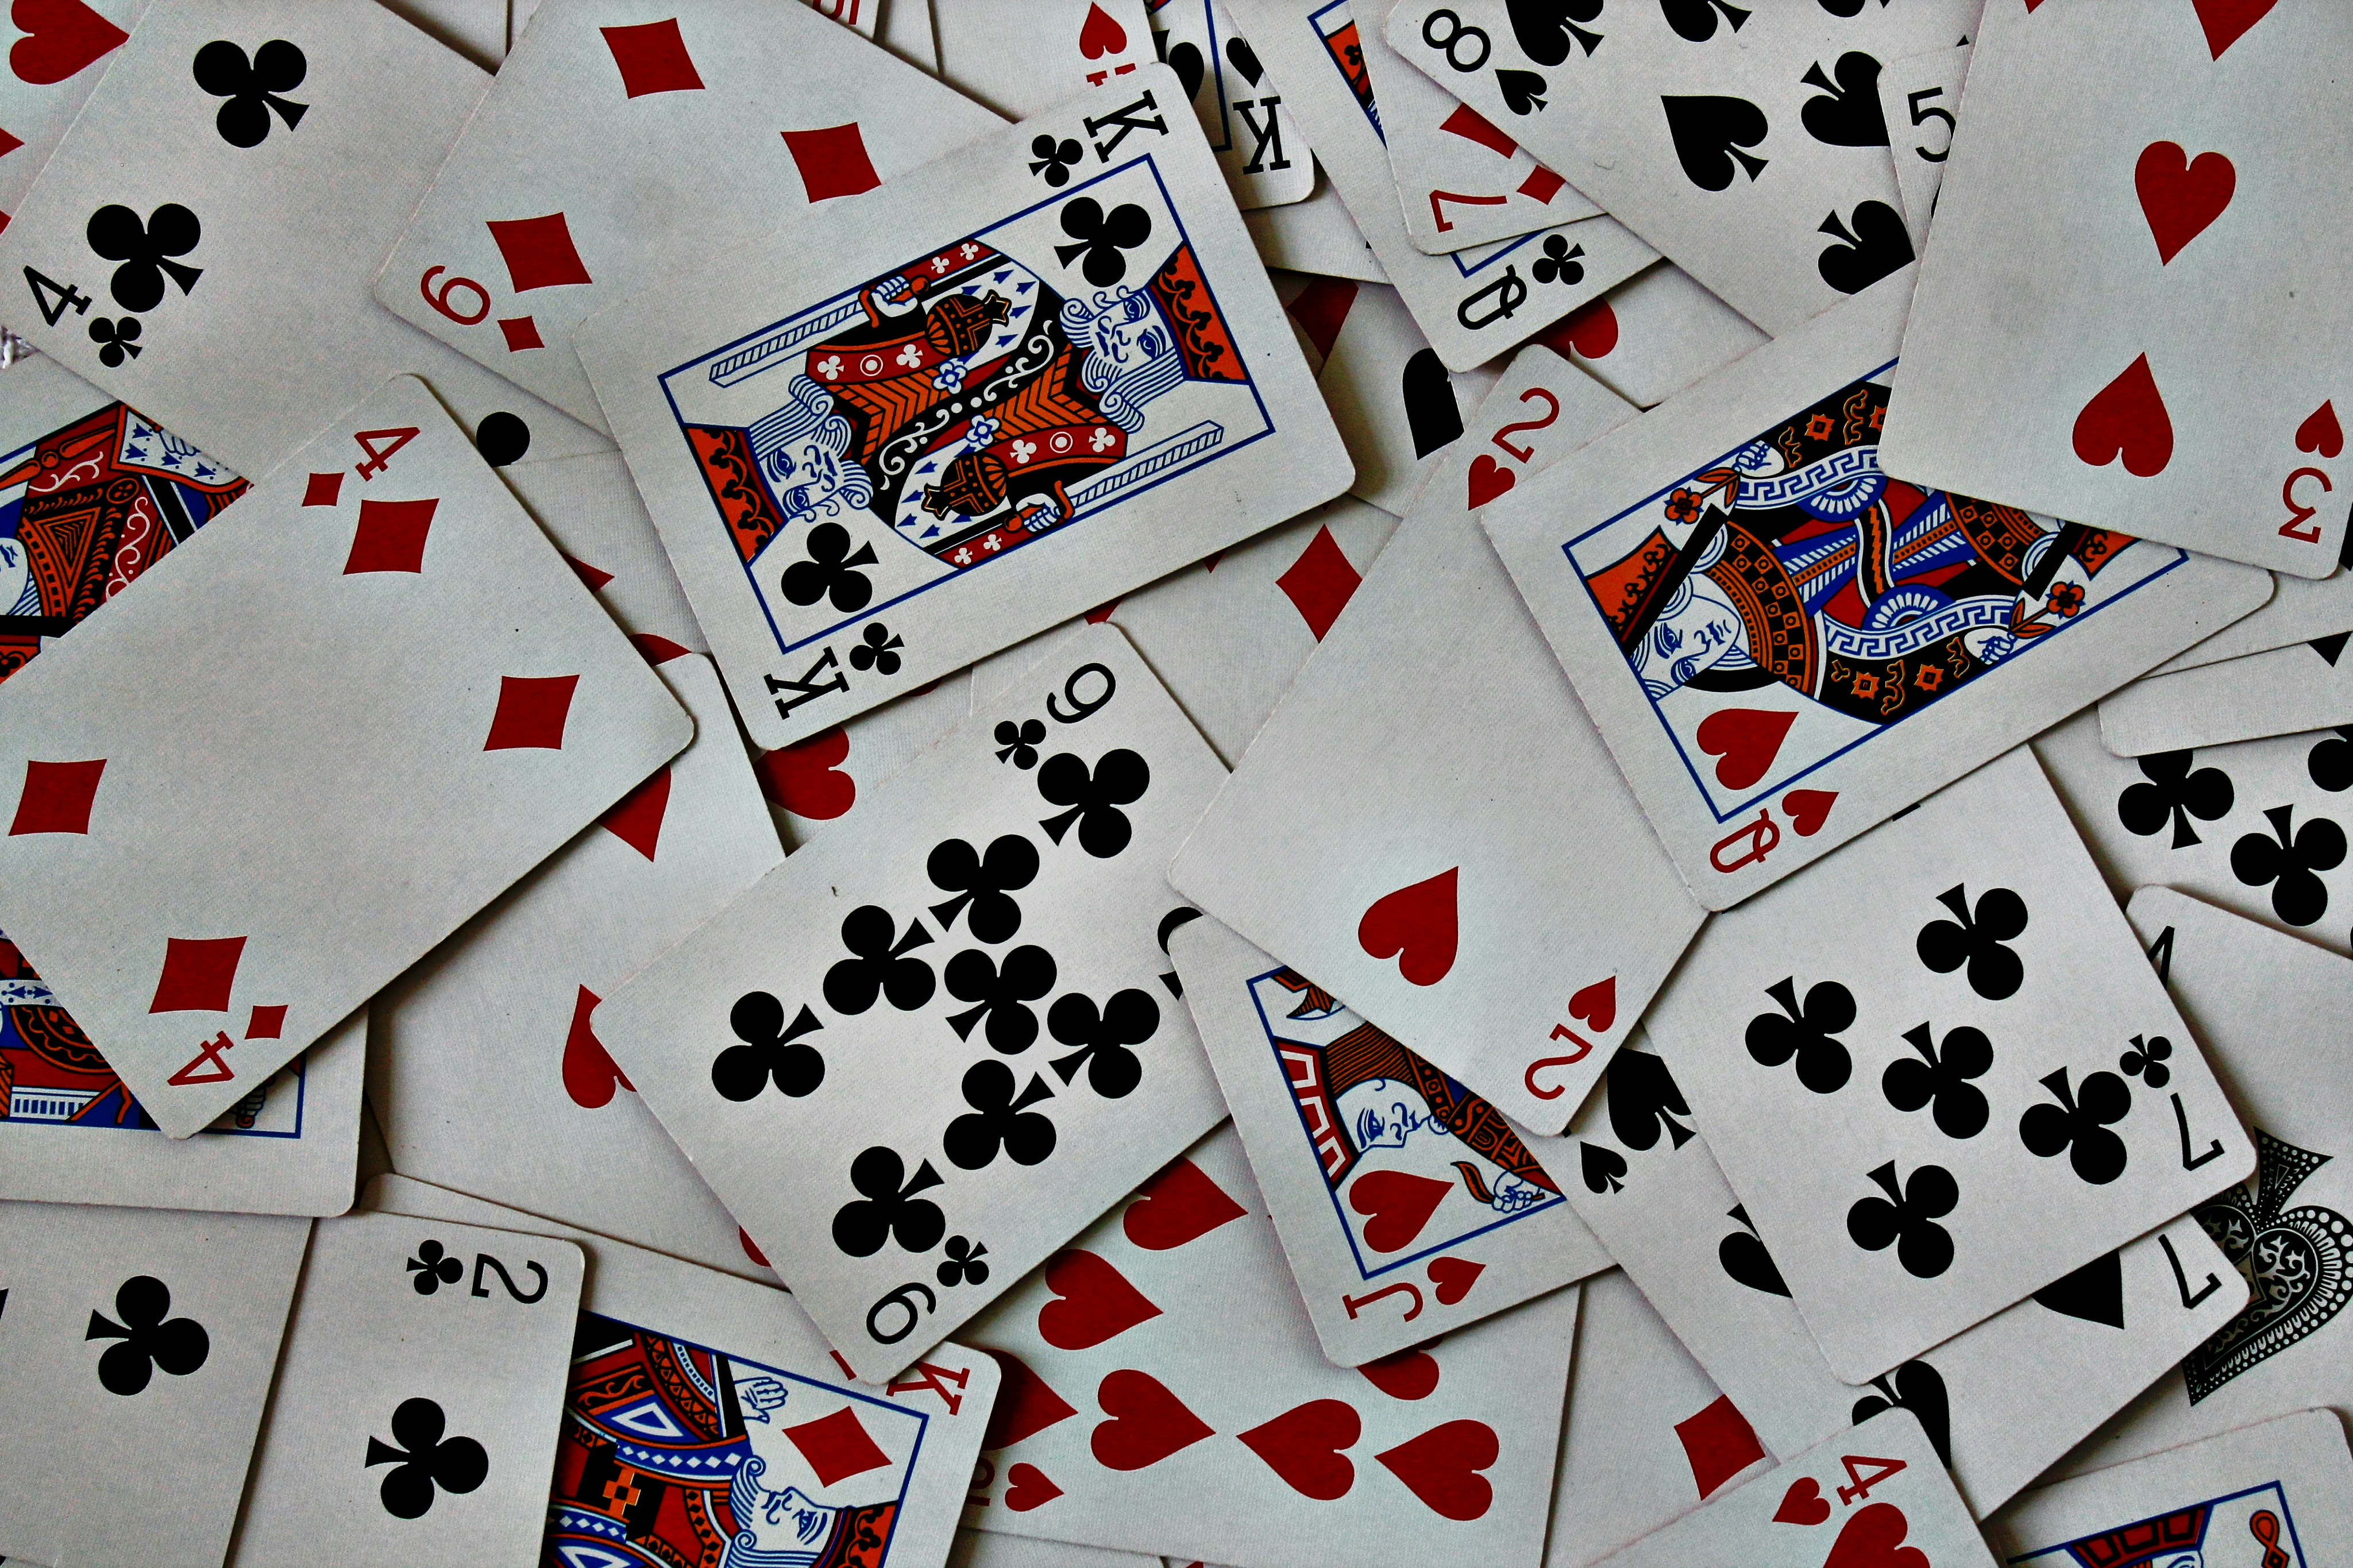
\includegraphics[width=0.7\linewidth]{imagens/Cartas.jpg}
	\\\textbf{Fonte:} \url{https://unsplash.com/pt-br/fotografias/uma-pilha-de-cartas-de-baralho-sentadas-umas-em-cima-das-outras-P787-xixGio}
	\label{fig:cartas}
\end{figure}
\FloatBarrier


\subsection{Jogos Atléticos}


Há também os jogos atléticos, uma das formas mais tradicionais de jogos, que destaca a destreza física em detrimento das habilidades mental e possuem regras que especificam estritamente as ações que o jogador pode ou não realizar. Tais jogos estão em uma linha tênue com as competições atléticas, sendo distinguidos pelo grau de interação entre os jogadores \cite{Crawford1997}. Na Figura~\ref{fig:futebol} há um exemplo de jogo atlético, o futebol.


\FloatBarrier 
\begin{figure}[!htbp]
	\centering
	\caption{Jogo de futebol}
	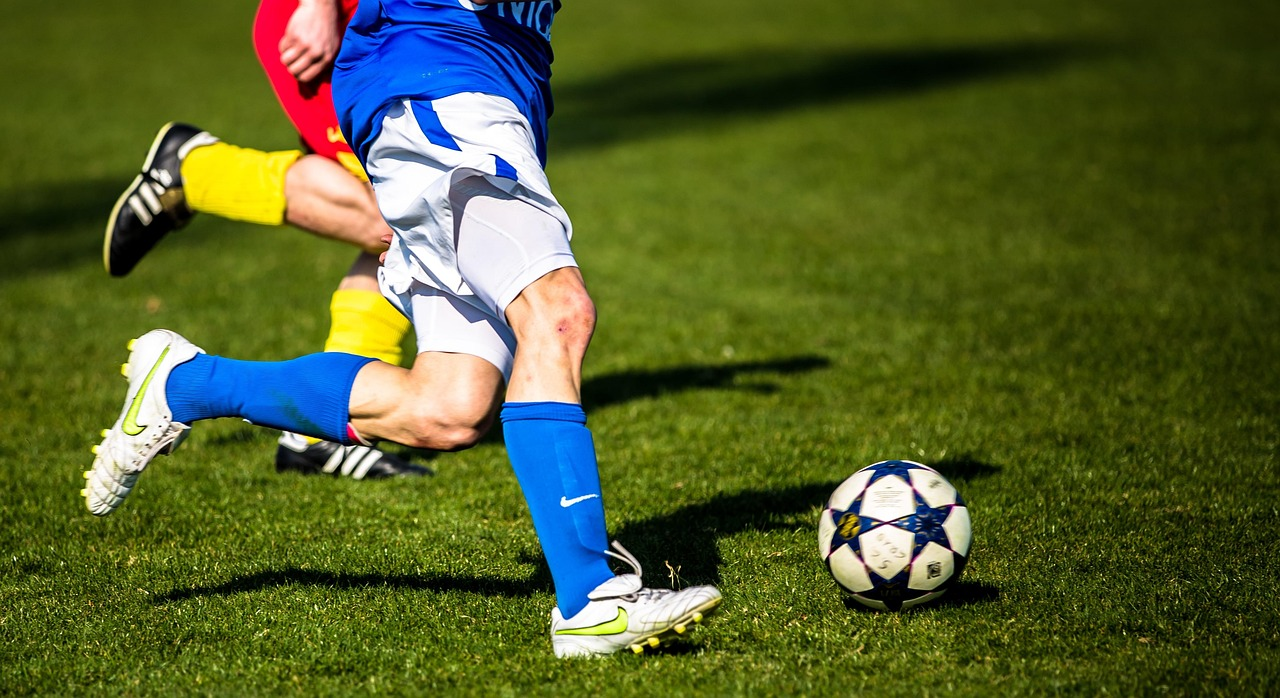
\includegraphics[width=0.7\linewidth]{imagens/futebol.jpg}
	\\\textbf{Fonte:} \url{https://pixabay.com/pt/photos/futebol-duelo-grama-bola-esportes-1331838/}
	\label{fig:futebol}
\end{figure}
\FloatBarrier



\subsection{Jogos Digitais}


Por fim, temos os jogos digitais, os mais populares atualmente e a categoria central deste trabalho. Esses jogos se adequam a diferentes tipos de computadores e plataformas, incluindo máquinas dedicadas, como os fliperamas, consoles domésticos, computadores pessoais e dispositivos portáteis, como o \textit{Nintendo DS} ou até mesmo os celulares \cite{Crawford1997}.


\section{Tipos de Jogos Eletrônicos}

Segundo a definição de \citeauthorandyear{Juul2005}, pesquisador dinamarquês reconhecido na área de \textit{game studies}, os jogos eletrônicos são definidos como uma combinação de regras reais inseridas em mundos fictício, com os quais os jogadores interagem. Essa interação não se limita apenas às mecânicas dos jogos; ela se manifesta em diversos aspectos, incluindo seu design, bem como a forma que os jogos são interpretados, utilizados e discutidos.

No entanto, essa definição desconsidera aspectos culturais nos quais o jogo está inserido, focando apenas na estrutura interna do jogo. E a partir disso, \citeauthorandyear{Apperley2006}, teórico da mídia digital e pesquisador dos estudos de jogos, propõe uma abordagem alternativa, categorizando os videogames com base em como eles são jogados e recebidos. Essa proposta compreende os jogos a partir das práticas sociais e culturais, enfatizando a experiência prática e situada do jogador.

A categorização dos videogames de \citeauthorandyear{Apperley2006} será apresentada a seguir.


\subsection{Simulação}

Embora todos os jogos sejam, de certa forma, simulações, os jogos de simulação buscam representar claramente uma atividade do mundo real, sendo relacionadas a esportes, voos e direção, ou até mesmo simular a dinâmica de cidades e vilarejos. A maior parte desses jogos se encaixam na noção de remediação, pois sua jogabilidade é reaproveitada de atividades relativamente comuns ou representadas nas mídias. Um exemplo popular é o jogo \textit{Euro Truck Simulator}, que simula a direção de um caminhão, apresentada na Figura~\ref{fig:simulacao}.


\FloatBarrier 
\begin{figure}[!htbp]
	\centering
	\caption{\textit{Euro Truck Simulator}}
	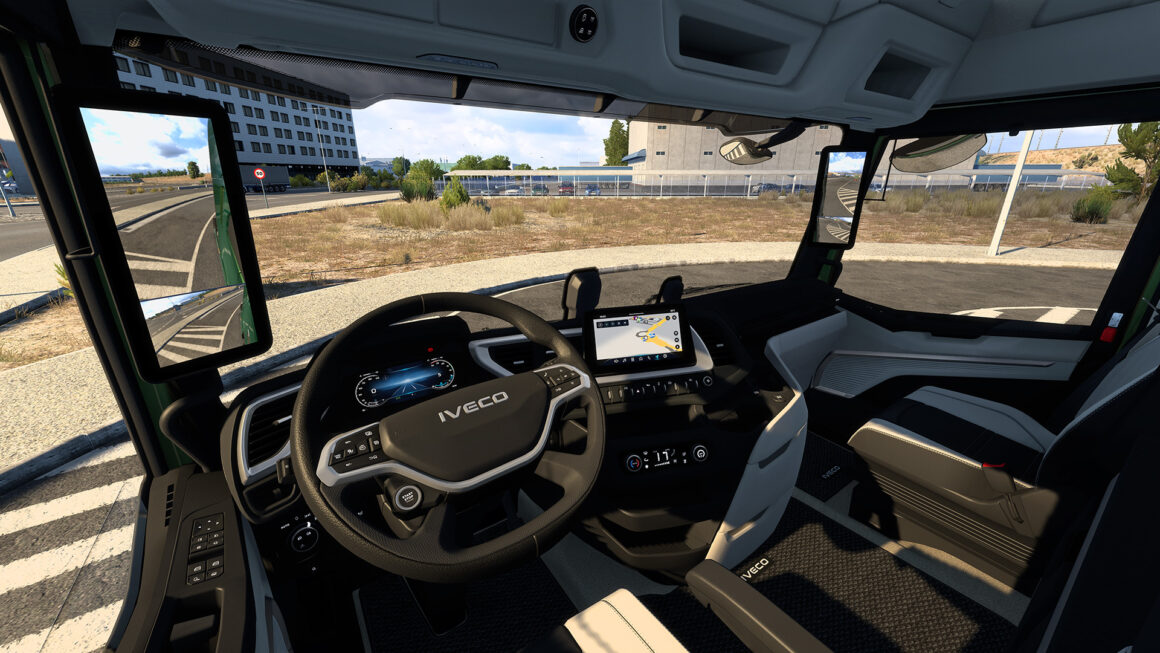
\includegraphics[width=0.7\linewidth]{imagens/EuroTruck.jpg}
	\\\textbf{Fonte:} \url{https://estradao.estadao.com.br/caminhoes/caminhao-pesado-iveco-s-way-estreia-no-euro-truck-simulator-2/ }
	\label{fig:simulacao}
\end{figure}
\FloatBarrier


\subsection{Estratégia}

Os jogos de estratégia são caracterizados pelo planejamento e pela tomada de decisões táticas. Geralmente são divididos em dois subgêneros: a estratégia em tempo real (RTS) e baseada em turnos (TBS). Ambos possuem uma estética semelhante, sendo tendentes a um conceito fotorrealista. Tais jogos priorizam a gestão de recursos, o pensamento analítico e a adaptação estratégica, exigindo, assim, uma atenção profunda do jogador. Um exemplo de TBS é o jogo \textit{Teamfight Tactics (TFT)} apresentado na Figura~\ref{fig:tactics}.

\FloatBarrier 
\begin{figure}[!htbp]
	\centering
	\caption{\textit{Teamfight Tactics (TFT)}}
	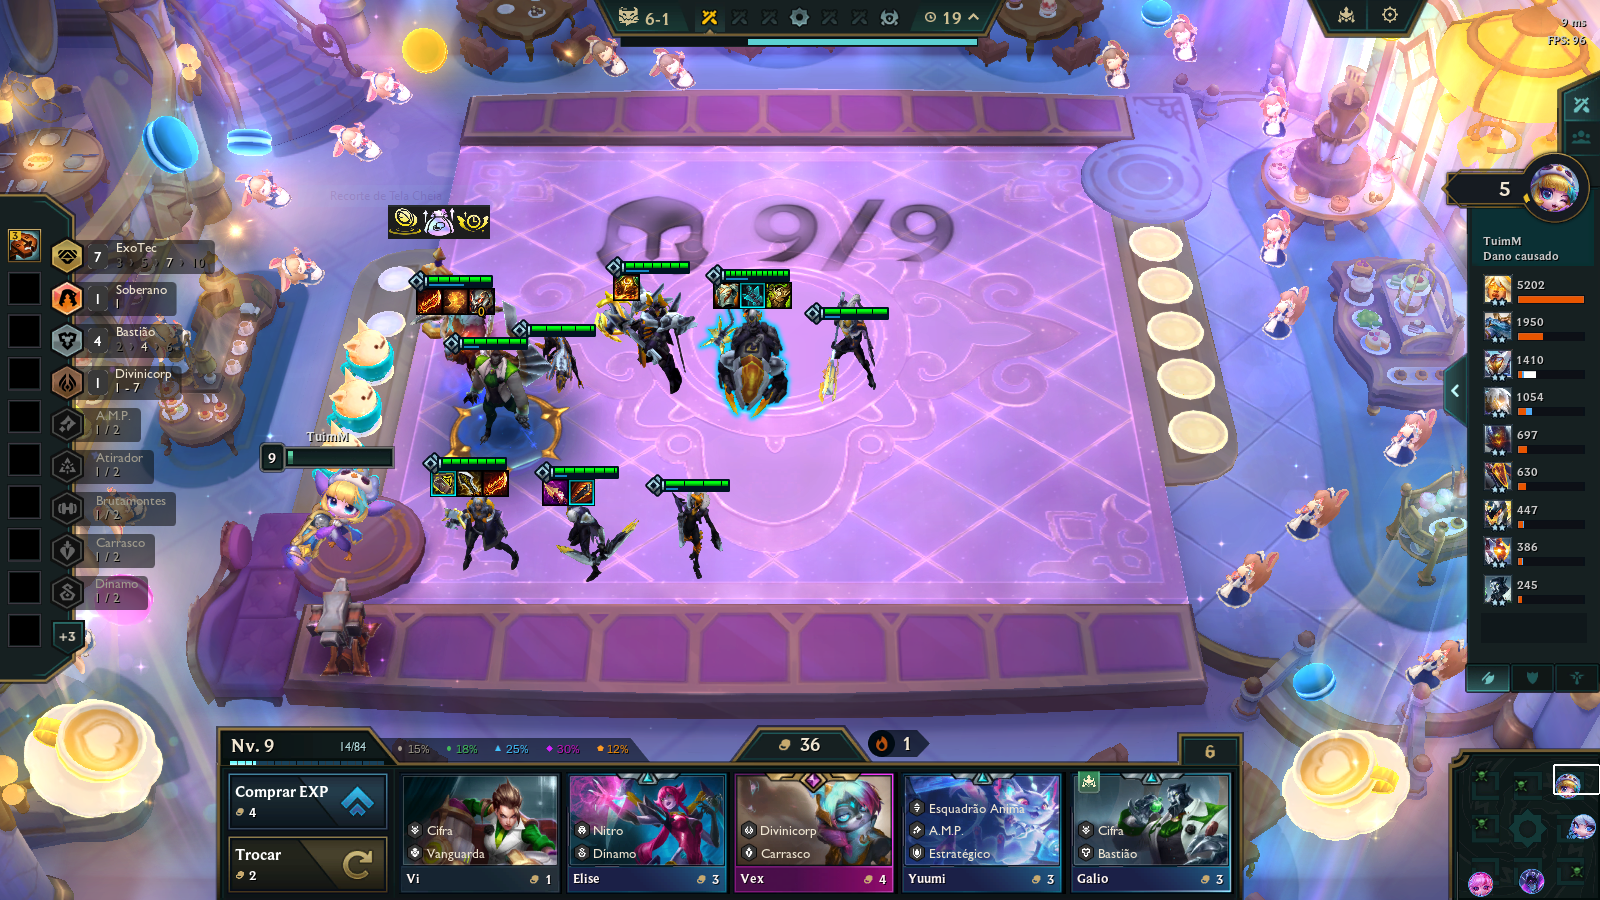
\includegraphics[width=0.7\linewidth]{imagens/tft3.png}
	\\\textbf{Fonte:} Elaborada pelo autor
	\label{fig:tactics}
\end{figure}
\FloatBarrier


\subsection{Ação}

Assim como os jogos de estratégia, os jogos de ação também podem ser divididos em dois subgêneros: jogos de tiro em primeira pessoas, conhecidos como FPS (\textit{First Person Shooters}), nos quais a câmera simula a própria visão do jogador, e jogos em terceira pessoa, que representam o personagem totalmente visível na tela, geralmente visto por trás. Tais jogos priorizam a agilidade, precisão e o tempo de reação do jogador, oferecendo experiências intensas e dinâmicas. Um FPS popular é o jogo \textit{Valorant} apresentado na Figura~\ref{fig:vava}.


\FloatBarrier 
\begin{figure}[!htbp]
	\centering
	\caption{\textit{Valorant}}
	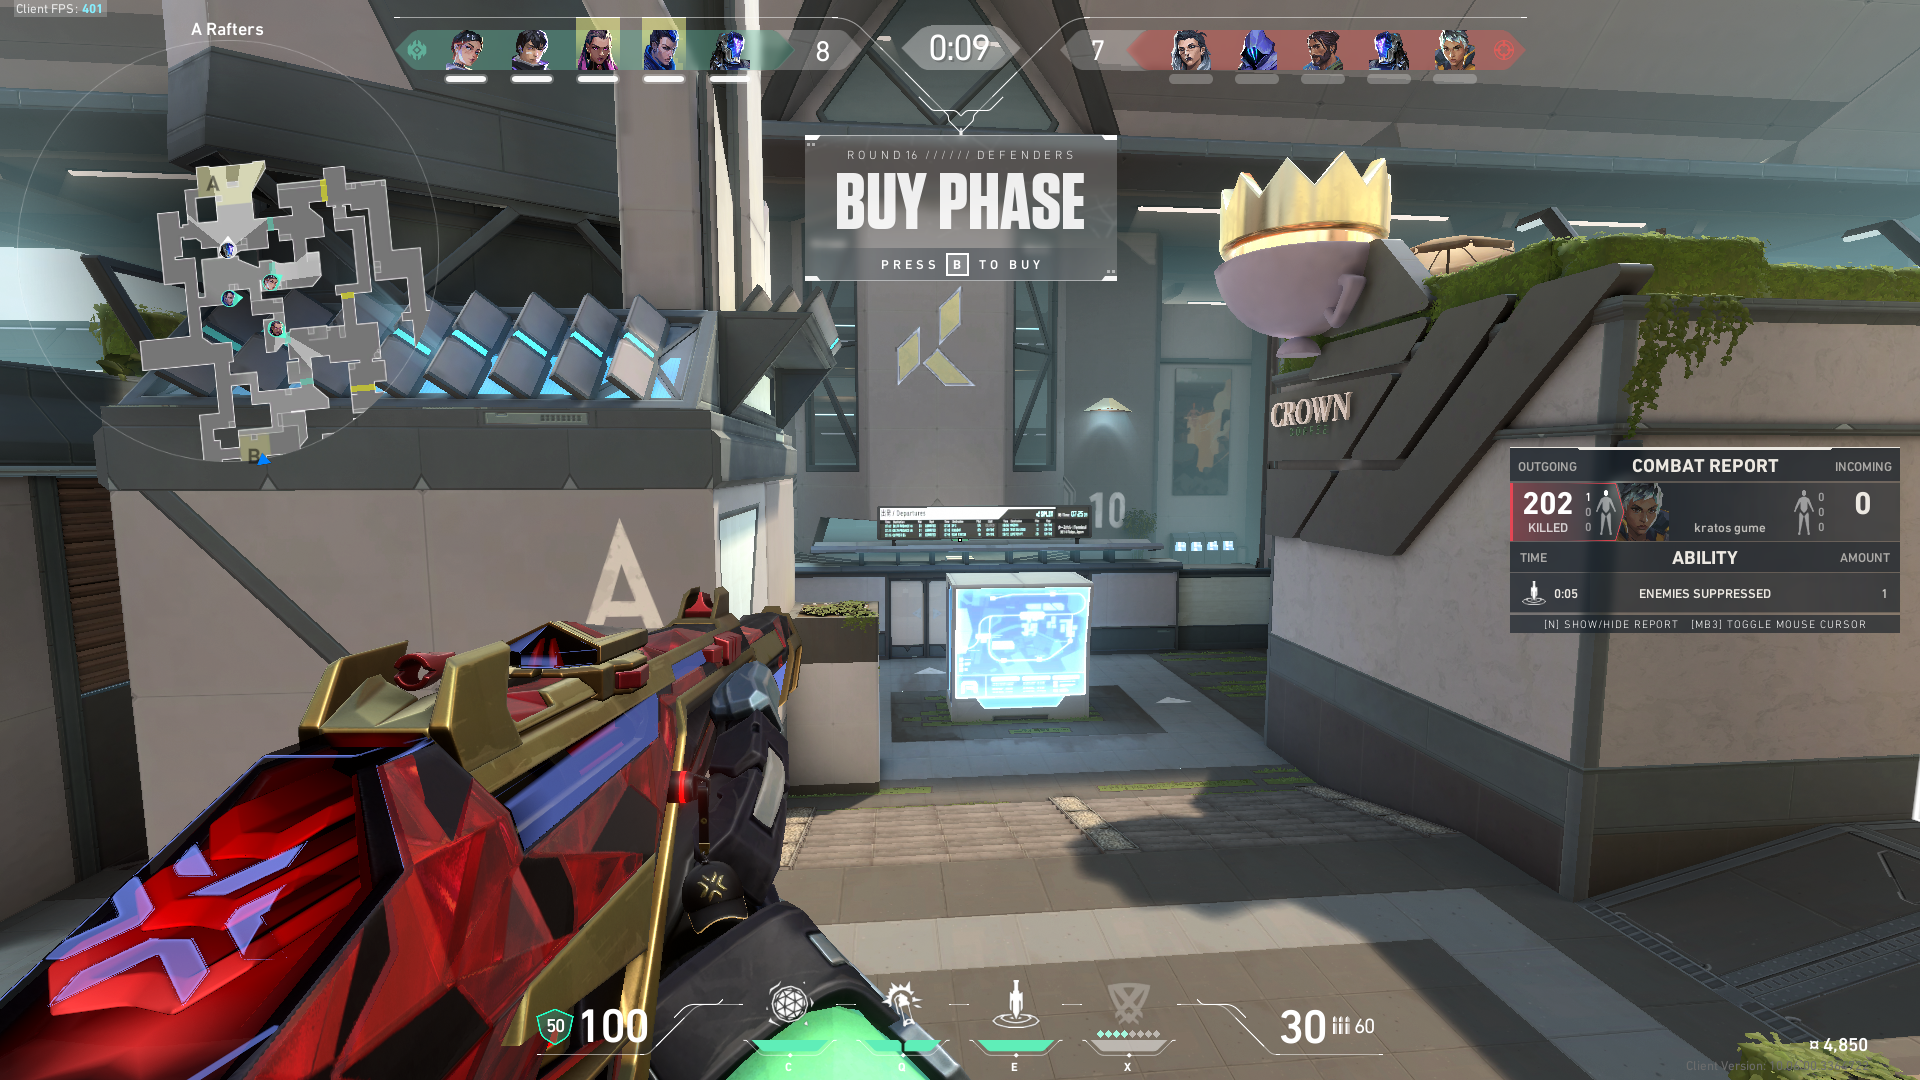
\includegraphics[width=0.7\linewidth]{imagens/valorant.png}
	\\\textbf{Fonte:} Elaborada pelo autor
	\label{fig:vava}
\end{figure}
\FloatBarrier


\subsection{\textit{Role-playing}}

Nos jogos de \textit{Role-playing}, ou RPGs, os jogadores interpretam seus personagens em mundos fictícios, narrando suas ações a um mestre, o qual conduz os resultados dessas ações. Originados do clássico  \textit{Dungeons and Dragons} na década de 1970 \cite{Mason2004}, esse jogos evoluíram para versões digitais, mantendo elementos como a progressão de personagens, porém agora limitando a improvisação e focando em desafios mecânicos e uma narrativa mais centrada.

\section{Tecnologias para Desenvolvimento de Jogos} 

O código-fonte de um jogo é, sem dúvida, seu elemento central, incluindo tudo que está diretamente relacionado ao jogo, definindo a experiência do jogador, como a jogabilidade, os elementos visuais, sistema de pontuação, entre outros aspectos \cite{Rabin2021}. Embora seja possível criar um jogo utilizando puramente linguagens de programação, como \textit{Java}, \textit{C} ou até mesmo bibliotecas como \textit{Raylib}, o uso de uma \textit{engine} pode facilitar o desenvolvimento e garantir uma maior eficiência na produção de um jogo.

De acordo com a definição de \citeauthorandyear{CluaBittencourt2005}, uma \textit{engine}, ou motor gráfico, é uma ferramenta essencial no desenvolvimento de jogos, responsável por executar diversas funcionalidades técnicas. Entre elas estão o \textit{hardware} gráfico, o controle dos modelos a serem renderizados e o tratamento das entradas de dados do jogador. Além disso, ela lida com os processos básicos que garantem o funcionamento adequado do jogo. 

\subsection{Godot}

A \textit{Godot} é uma \textit{engine} de código aberto, totalmente independente e conduzida pela comunidade, com o apoio da fundação \textit{Godot Foundation}. Trata-se de uma \textit{engine} multiplataforma que suporta criação de jogos 2D e 3D, oferece um conjunto abrangente de ferramentas integradas, proporcionando aos desenvolvedores uma maior praticidade. Além disso, ela promove uma facilidade de exportação para diversas plataformas, como sistemas \textit{desktop}, dispositivos móveis e consoles  \cite{GodotDocs2024}.

De acordo com o desenvolvedor de jogos e escritor \citeauthorandyear{Bradfield2018}, a Godot é uma \textit{engine} moderna e completa, tendo como diferencial o fato de a ferramenta ser totalmente gratuita e distribuída sob a licença MIT, a qual assegura aos desenvolvedores liberdade total sobre seus projetos. Tal atrativo distingue a \textit{Godot} das demais \textit{engine}, as quais estabelecem restrições contratuais ou cobranças sobre a porcentagem dos lucros obtidos com os jogos criados.


Além desses benefícios, a \textit{Godot} possui sua própria linguagem de programação, a  \textit{GDScript}. Desenvolvida especialmente para a \textit{engine}, ela oferece uma sintaxe simples, sendo semelhante à do Python, e permite uma integração total com o editor. A \textit{GDScript} foi criada com foco em desempenho e produtividade, evitando limitações comuns encontradas em outras linguagens de uso geral no desenvolvimento de jogos.\cite{GodotDocs2024}.

Na Figura~\ref{fig:godot} é apresentado a interface da \textit{engine Godot}.

\FloatBarrier 
\begin{figure}[!htbp]
	\centering
	\caption{\textit{Interface Godot}}
	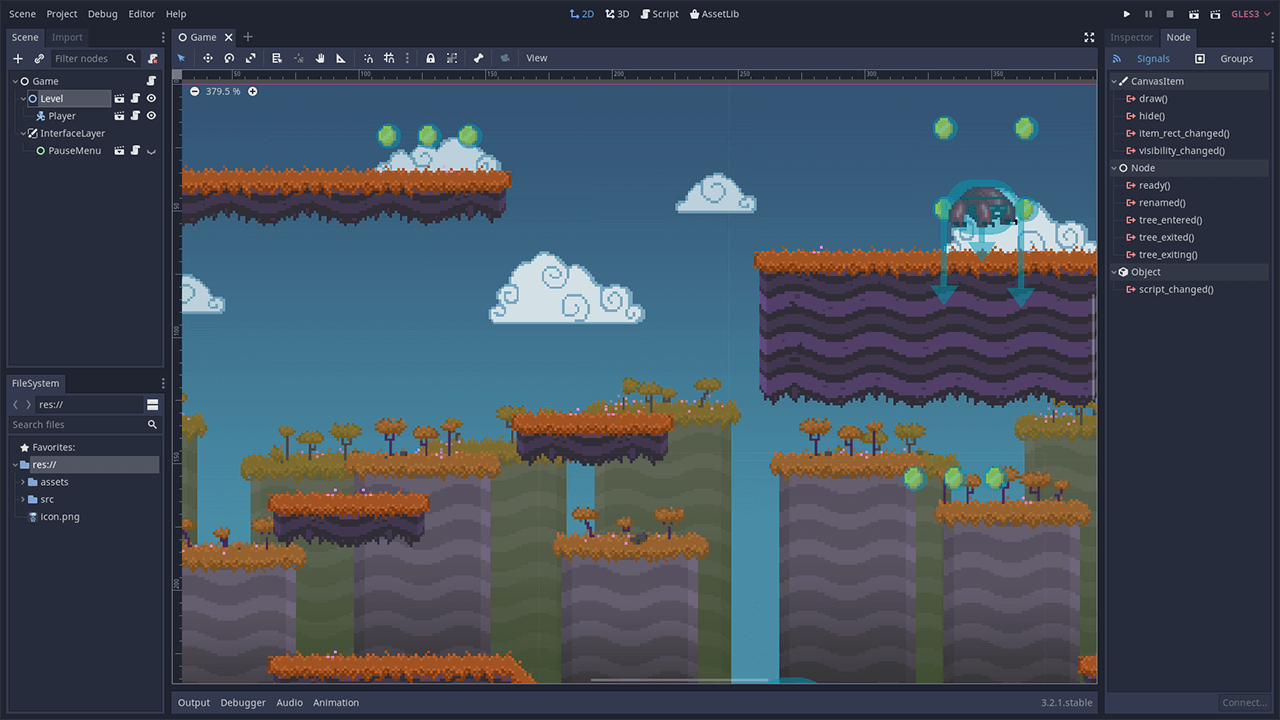
\includegraphics[width=0.7\linewidth]{imagens/godot-editor-01.png}
	\\\textbf{Fonte:} \url{https://videogamewarlock.com/godot-engine-desenvolva-games-com-liberdade/} 
	\label{fig:godot}
\end{figure}
\FloatBarrier


\subsection{Unity}

A \textit{Unity} é um motor de jogos multiplataformas amplamente utilizado no desenvolvimento de jogos 2D e 3D, assim como na criação de visualizações e simulações interativas. É considerada um dos motores mais populares entre os desenvolvedores, devido sua facilidade de uso, flexibilidade e eficiência. Seu ambiente de desenvolvimento disponibiliza diversos recursos integrados, como o \textit{Adaptive Performance} e o suporte à programação em C\#, que possibilitam a criação de jogos com alto desempenho e qualidade \cite{Hussain2020}.

A empresa \textit{Unity Technologies } é a responsável pelo desenvolvimento da \textit{Unity}, cuja primeira versão foi lançada em 2005, durante a conferência da \textit{Apple}. Inicialmente, essa versão era voltada somente para o desenvolvimento no sistema OS X, visando tornar a criação de jogos mais acessível. Atualmente, a \textit{Unity} evoluiu e oferece suporte para certa de 27 plataformas  incluindo dispositivos móveis, desktops, consoles, navegadores e realidade virtual \cite{Smid2017}.

Na Figura~\ref{fig:unity} é apresentado a interface da \textit{engine Unity}.

\FloatBarrier 
\begin{figure}[!htbp]
	\centering
	\caption{\textit{Interface Unity}}
	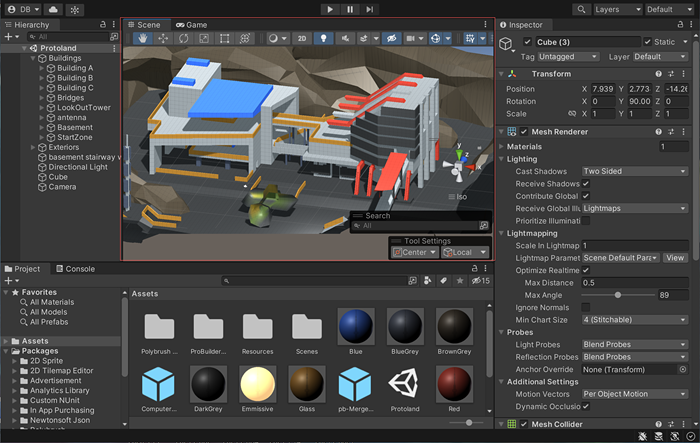
\includegraphics[width=0.7\linewidth]{imagens/unity.png}
	\\\textbf{Fonte:}\url{https://docs.unity3d.com/Manual/UsingTheSceneView.html } 
	\label{fig:unity}
\end{figure}
\FloatBarrier



\subsection{Unreal Engine}

\textit{Unreal Engine} é um motor gráfico desenvolvido pela empresa \textit{Epic Games} e, atualmente, é considerada a principal \textit{engine} para visualizações realistas, e a criação de vegetação e terrenos. É a \textit{engine} mais indicada para projetos grandes e, embora possua suporte para \textit{IOS} e \textit{Android}, não é a mais recomendada para jogos \textit{mobile}. Um de seus maiores diferencias é o sistema \textit{Blueprint}, uma ferramenta visual de lógica composta por grafos conectados através de blocos, substituindo a necessidade de \textit{scripts} tradicionais \cite{Smid2017}.

Também de acordo com o acadêmico \citeauthorandyear{Smid2017}, a \textit{Unreal Engine} utiliza da linguagem de programação C++, tanto para implementação dos jogos quanto para o desenvolvimento de seu código-fonte aberto, proporcionando assim um grande controle sobre o sistema para os usuários. Além disso, sua tecnologia de renderização é muito eficaz, possuindo efeitos de pós-processamento rápidos com diversos recursos integrados. A \textit{engine} também dispõe de um editor para a criação de  materiais personalizados, e ferramentas para otimização e depuração visual.

Na Figura~\ref{fig:unreal} é apresentado a interface da \textit{Unreal Engine}.

\FloatBarrier 
\begin{figure}[!htbp]
	\centering
	\caption{\textit{Interface Unreal Engine}}
	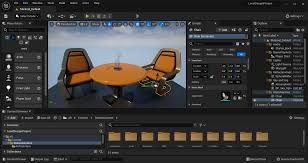
\includegraphics[width=0.7\linewidth]{imagens/unreal.jpg}
	\\\textbf{Fonte:}\url{https://dev.epicgames.com/community/learning/tutorials/PnXj/unreal-engine-in-development-overview-of-the-unreal-editor-interface} 
	\label{fig:unreal}
\end{figure}
\FloatBarrier


\subsection{Game Maker}	

\textit{Game Maker} é uma \textit{engine} de desenvolvimento multiplataforma
criada pela \textit{YoYo Games}. Ela possui sua própria linguagem de \textit{script}, a \textit{Game Maker Language}, além de oferecer uma linguagem visual baseada no sistema de arrastar e soltar. Por conta desta tecnologia, o \textit{Game Maker} se destaca como uma excelente \textit{engine} para desenvolvedores iniciantes, e embora seja voltada principalmente para a criação de jogos 2D, tambem é possivel o desenvolvimento de jogos 3D \cite{Sparks2020}.

Além das ferramentas já mencionada, a \textit{engine} também oferece um editor de imagens completo, para a criação e edição de \textit{sprites} diretamente da plataforma. Também é possível importar arquivos externos, como animações e imagens vetorizadas, conta com editores para manipulação de objetos, salas, sequências animadas e outros recursos que facilitam o desenvolvimento de jogos \cite{GameMakerManual2023}. 

Na Figura~\ref{fig:gamemaker} é apresentado a interface do \textit{Game Maker}.

\FloatBarrier 
\begin{figure}[!htbp]
	\centering
	\caption{\textit{Interface Game Maker}}
	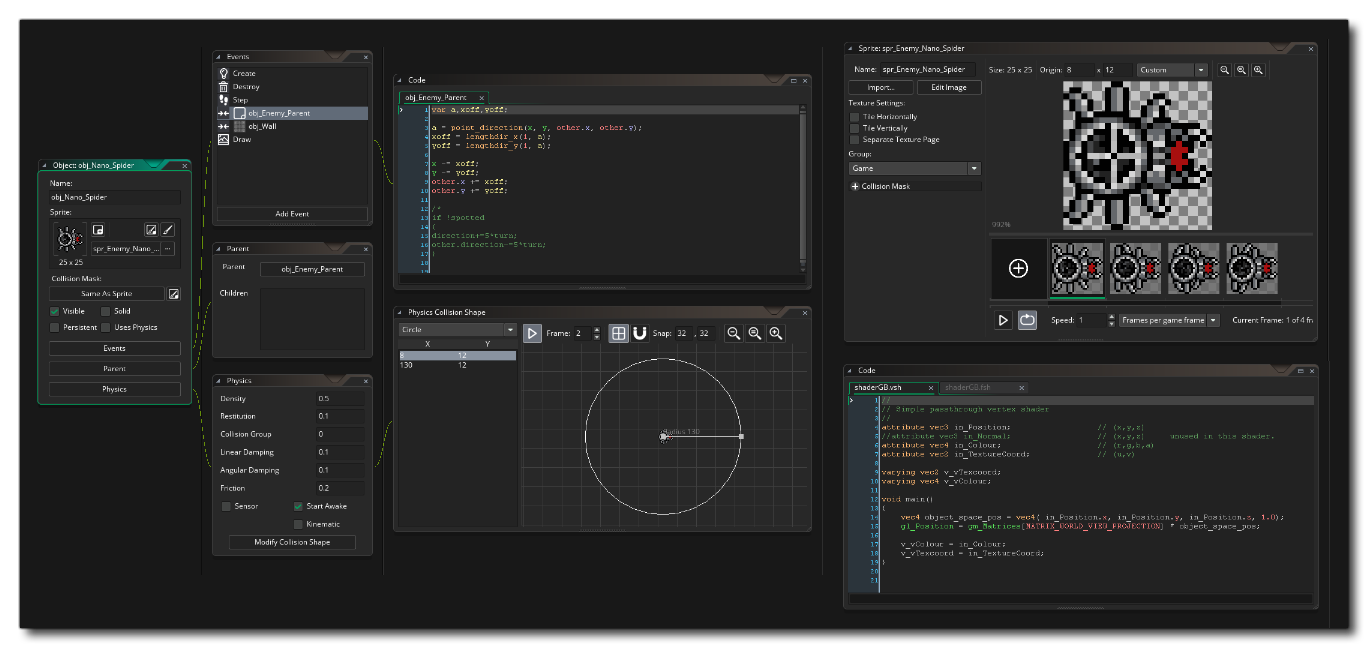
\includegraphics[width=0.7\linewidth]{imagens/gamemaker.png}
	\\\textbf{Fonte:} \url{	https://manual.gamemaker.io}
	\label{fig:gamemaker}
\end{figure}
\FloatBarrier


\section{Trabalhos Correlatos}


\subsection{Luxos Adventure}

\citeauthorandyear{cordeiro2023} inicia seu trabalho apresentando uma contextualização sobre o mundo dos jogos atuais e demonstra as etapas para a criação de seu jogo, \textit{Luxos Adventure}, um RPG 2D em estilo top-down, com elementos de ação e \textit{roguelike}. Foi utilizada a \textit{engine Godot}, destacando o uso da mesma por se tratar de uma \textit{engine} gratuita, de código aberto com suporte tanto para jogos 2D quanto 3D. A mesma foi escolhida por conta da facilidade no uso e por sua popularidade entre desenvolvedores independentes.

O trabalho explora desde a concepção inicial da jogo até o desenvolvimento prático, possuindo etapas como a elaboração do \textit{Game Design Document }(GDD), a implementação do \textit{assets}, o desenvolvimento da lógica de jogo, a construção de cenas e a animação dos personagens. O projeto se destaca por demonstrar, de forma prática, como é possível desenvolver um jogo funcional e bem estruturado, unindo criatividade, pesquisa e conhecimentos técnicos em desenvolvimento de jogos.


\subsection{Speedy Dungeon}

Em seu estudo, \citeauthorandyear{silva2022} apresentou o processo de desenvolvimento do jogo \textit{Speedy Dungeon}, um jogo no estilo \textit{dungeon crawler} 2D desenvolvido na \textit{engine Godot}. O autor define o conceito e elabora o \textit{Game Design Document }(GDD) para, em seguida, configurar o ambiente de desenvolvimento a criação dos primeiros protótipos. Utiliza a estrutura em nós da Godot para organizar o cenário, movimentação do personagem, lógica de combate e elementos de interface. O projeto demonstra o uso da Godot no desenvolvimento de jogos independentes, destacando sua flexibilidade e recursos para criação de jogos.

\subsection{Desenvolvimento de um jogo 2D utilizando Unity}

\citeauthorandyear{sofiatti2022} descreve em seu trabalho o desenvolvimento de um jogo 2D de plataforma denominado \textit{Forest Path}, utilizando a \textit{engine Unity} e com foco na aplicação dos conhecimentos  em desenvolvimento de jogos. O projeto explora desde a contextualização histórica dos jogos até a escolha da engine, justificando a opção pela Unity por sua popularidade, facilidade de uso e suporte a jogos 2D. Além disso, apresenta o levantamento de requisitos, a criação do GDD e a implementação dos elementos visuais, lógicos e funcionais, como sprites, animações, movimentação e combate, utilizando \textit{assets} gratuitos e \textit{scripts} em C\#.

\chapter{Metodologia}
\label{cap:03}

O processo de desenvolvimento de um jogo pode ser realizado de diversas formas, dependendo do tipo de jogo a ser criado. Neste trabalho, o desenvolvimento será baseado no diagrama apresentado na figura~\ref{fig:metodologia}, que apresenta todas as etapas do processo de criação do jogo proposto.

\FloatBarrier 
\begin{figure}[!htbp]
	\centering
	\caption{\textit{Diagrama de metodologia}}
	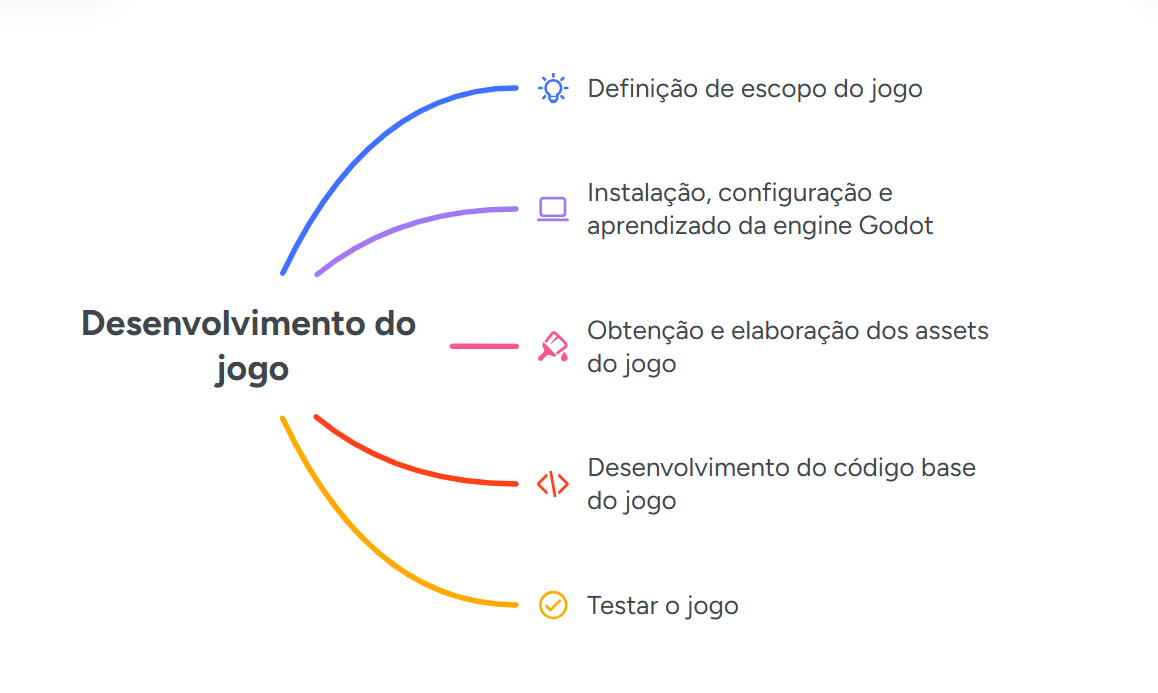
\includegraphics[width=1 \linewidth]{imagens/metodologia.png}
	\\\textbf{Fonte:} Elaborada pelo autor
	\label{fig:metodologia}
\end{figure}
\FloatBarrier


\section{Definição do escopo do jogo}

A definição do escopo uma etapa primordial no desenvolvimento de qualquer jogo, pois orienta as demais fases do projeto. Nessa etapa, será definido o gênero do jogo que será criado e, a partir disso, serão elaboradas as mecânicas, os elementos visuais e demais componentes que darão forma à experiência do jogador. Neste trabalho optou-se pelo desenvolvimento de um \textit{cozy game} em 2D, com o objetivo de proporcionar uma experiência relaxante e acolhedora ao jogador.	

\section{Processo de Instalação, Configuração e Aprendizado da Engine Godot}

O ambiente de desenvolvimento será preparado com o objetivo de tornar o processo mais eficiente em todas as etapas do projeto. Para isso, será escolhida a \textit{Godot Engine}, que se mostra uma boa opção por ser de fácil aprendizado e gratuita. A configuração envolve a instalação da \textit{engine}, a organização das pastas do projeto e o estudo da linguagem \textit{GDScript}. Essa organização inicial busca evitar problemas ao longo da criação do jogo.


\section{Elaboração do Game Design Document (GDD)}




\section{Obtenção e desenvolvimento dos assets do jogo}

Os \textit{assets} são todos os recursos que serão 	utilizados na construção do jogo, podendo ser imagens, efeitos sonoros e músicas. Os \textit{sprites}, elementos básicos que foram utilizados para representar o personagem principal, dando efeito de animação ao mesmo, e para compor o cenário, serão obtidos gratuitamente através do site \textit{itch.io}. Além disso, serão elaborados outros \textit{sprites} para complementar o projeto.

\section{Desenvolvimento do código-base do jogo}

No desenvolvimento do código-base do jogo, serão implementadas as mecânicas principais do personagem, a interface do usuário e outras funcionalidades essenciais para a execução do jogo. Além disso, nessa etapa ocorre a integração dos elementos visuais e sonoros, dando ao jogo uma atmosfera mais coerente e funcional.

\section{Testar o jogo}

Por fim, há a necessidade de realizar testes em todas as funções do jogo, garantido que não haja nenhum \textit{bug} ou erro no código que comprometa a execução do jogo. Também será verificado se todos os requisitos foram atendidos e o jogo funciona conforme o esperado.
\chapter{Análise dos Resultados}
\label{cap:04}

Relatar os resultados obtidos a partir dos experimentos e dos estudos realizados. 


\section{Resultados/Impactos}

Resultados.


\section{Orçamento}

Orçamento, caso exista.


\section{Cronograma do Trabalho}

Segue abaixo o cronograma de trabalho das atividades realizadas e das que serão executadas até a Avaliação Final de TCC.

\textbf{Obs:} Para facilitar, crie o cronograma usando o modelo do Word contido no projeto (imagens/templateCronograma.docx), ou qualquer outro \textit{software}, salve a imagem e atualize o arquivo imagens/cronograma.png.

\FloatBarrier
\begin{figure*}[!htbp]
	\centering
	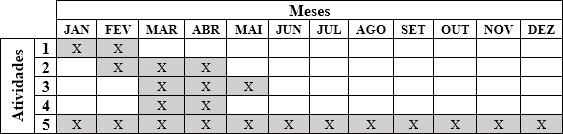
\includegraphics[scale=1]{imagens/cronograma}
\end{figure*}
\FloatBarrier

\begin{enumerate}
	\item Descrição da atividade 1;
	\item Descrição da atividade 2;
	\item Descrição da atividade 3;
	\item Descrição da atividade 4;
	\item Descrição da atividade 5.
\end{enumerate}

\chapter{Conclusões e Recomendações}
\label{cap:05}

São descritas claramente as conclusões retiradas das discussões e dos experimentos realizados no decorrer da pesquisa, e finalizada a parte textual do trabalho. Recomendações são declarações concisas de ações, julgadas necessárias a partir das conclusões obtidas, a serem usadas no futuro. Ou seja, lembre-se de apresentar os possíveis trabalhos futuros derivados do seu trabalho.


% ----------------------------------------------------------
% Referências bibliográficas
% ----------------------------------------------------------
\postextual
\bibliography{referencias}

\end{document}
